\section{误差与收敛}
\label{sec:odenum-error-convergence}

前两节看到的现象是：一步误差为$h^{p+1}$时，终点误差表现为$h^{p}$。数步数的算术说明不了这件事，因为早期产生的误差还要被后面的每一步继续传播，可能被放大。什么条件下这种累积可控？

\paragraph{一步局部误差的约定}
先把量纲说清楚。本书的局部截断误差~\eqref{eq:odenum-local-error}没有除以步长，它是一步之内产生的偏差，单位与状态相同。若方法的阶为$p$，它的大小是$O(h^{p+1})$。

有些文献把$\bm{\ell}^{(k+1)}/h$称为截断误差，这时阶为$p$的方法“局部截断误差”写作$O(h^{p})$。两种写法描述同一件事，读其他资料时要先确认定义。下表对比本章会用到的两个量。

\begin{BookInlineTable}
 \centering
 \caption{局部截断误差与全局误差的对比（阶为$p$的方法）。}
 \label{tab:odenum-local-global}
 \begin{tabular}{lll}
  \toprule
  & 局部截断误差$\bm{\ell}^{(k+1)}$ & 全局误差$\bm{e}^{(k)}$\\
  \midrule
  出发点 & 真解点$\bm{x}(t_k)$ & 实际算出的序列\\
  包含 & 一步更新的缺陷 & 全部历史的累积\\
  大小 & $O(h^{p+1})$ & 条件满足时$O(h^{p})$\\
  能否实际算出 & 需要真解 & 需要真解\\
  \bottomrule
 \end{tabular}
\end{BookInlineTable}

\paragraph{误差的传播图景}
式~\eqref{eq:odenum-error-split}说明每步的新误差与旧误差叠加。还可以换一个角度看：每步产生的偏差会被此后的真实流映射搬运到终点。把$\bm{\varphi}_{t,t_N}$作用于网格值，相邻两项之差就是第$k$步的贡献，它们相加后中间项全部抵消，在没有初值误差时得到
\begin{equation}
 \bm{e}^{(N)}=\sum_{k=0}^{N-1}\Bigl[\bm{\varphi}_{t_{k+1},t_N}\bigl(\bm{x}^{(k+1)}\bigr)-\bm{\varphi}_{t_k,t_N}\bigl(\bm{x}^{(k)}\bigr)\Bigr].
 \label{eq:odenum-telescoping}
\end{equation}

图~\ref{fig:odenum-error-fan}左侧画出这个分解。绿色折线是Euler网格值与真解之差，每个绿点处长出一条黄线，它是从该点出发的真解。相邻黄线在终点的间距，正是式~\eqref{eq:odenum-telescoping}的一项。

\begin{BookInlineFigure}
 \centering
 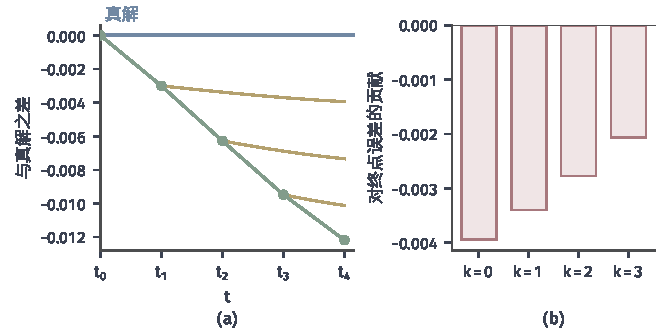
\includegraphics[width=112mm]{figures/06-differential-equations/01-ordinary-differential-equations/matplotlib/odenum-error-fan/figure.pdf}
 \caption{显式Euler方法的误差累积，问题为式~\eqref{eq:odenum-running}，$h=1/4$。(a)纵轴是与真解之差：蓝线是真解，绿线是网格值，黄线是从各网格值出发的真解。(b)式~\eqref{eq:odenum-telescoping}的四项，即每步偏差被搬运到$t=1$时的大小，四项之和等于终点误差$-0.01218$。}
 \label{fig:odenum-error-fan}
\end{BookInlineFigure}

例中四项依次为$-0.00394$、$-0.00340$、$-0.00277$、$-0.00206$，第一步的贡献最大。第一步本身的局部误差只有$-0.00300$，搬运到终点后变成$-0.00394$，因为这里$\partial_xf=1-2x>0$，邻近的解随时间分开。流映射放大扰动的程度决定了累积的结果，这与第~\ref{chap:ode-sensitivity}章的结论是同一回事。

\paragraph{一步稳定性}
要给出误差界，需要一个条件控制式~\eqref{eq:odenum-error-split}的第一项。连续情形的对应结论是Gronwall估计：若$\bm{f}$关于状态满足Lipschitz条件，常数为$L$，则从两个初值出发的解之差至多按$\mathrm{e}^{L(t-s)}$增长，推导见第~\ref{chap:ode-sensitivity}章。离散情形要求的是这种增长的一步版本。

数值解只需要在真解附近受控。取半径$\rho>0$，记真解周围的管状区域为
\begin{equation}
 \bm{K}_{\rho}=\bigl\{(t,\bm{y}):t\in[t_0,t_0+T],\ \lVert\bm{y}-\bm{x}(t)\rVert_2\leq\rho\bigr\}.
 \label{eq:odenum-tube}
\end{equation}

\begin{definition}[一步稳定性]
 \label{def:odenum-one-step-stability}
 设存在$\Lambda>0$和$h_0>0$，使当$0<h\leq h_0$时，对$\bm{K}_{\rho}$中所有同一时刻$t$的点$(t,\bm{y})$与$(t,\bm{z})$都有
 \begin{equation}
  \bigl\lVert\bm{\Psi}_h(t,\bm{y})-\bm{\Psi}_h(t,\bm{z})\bigr\rVert_2\leq(1+h\Lambda)\lVert\bm{y}-\bm{z}\rVert_2,
  \label{eq:odenum-one-step-stability}
 \end{equation}
 就称一步方法在$\bm{K}_{\rho}$上具有\term{一步稳定性}（one-step stability）。
\end{definition}

式中放大因子写成$1+h\Lambda$有明确的用意。走$N=T/h$步，累积因子至多是$(1+h\Lambda)^{T/h}\leq\mathrm{e}^{\Lambda T}$，不随$h\to0$增大。如果放大因子只是$1+\sqrt{h}$，下文会看到累积因子将趋于无穷。

这个条件可以逐个方法验证。设$\bm{f}$关于状态的Lipschitz常数在所考虑的区域上为$L$。显式Euler方法两点的差是
\[
 \bigl\lVert\bm{\Psi}_h(t,\bm{y})-\bm{\Psi}_h(t,\bm{z})\bigr\rVert_2
 \leq\lVert\bm{y}-\bm{z}\rVert_2+h\bigl\lVert\bm{f}(t,\bm{y})-\bm{f}(t,\bm{z})\bigr\rVert_2,
\]
第二项不超过$hL\lVert\bm{y}-\bm{z}\rVert_2$，所以$\Lambda=L$。

中点方法要多一层试探点。设$\bm{f}$在更大的管$\bm{K}_{2\rho}$上有界、Lipschitz常数为$L$，$h_0$足够小，使试探点仍在$\bm{K}_{2\rho}$内。两个点的第一个斜率之差不超过$L\lVert\bm{y}-\bm{z}\rVert_2$，第二个斜率之差满足
\[
 \lVert\bm{k}_2-\bm{k}_2'\rVert_2\leq L\Bigl(1+\frac{hL}{2}\Bigr)\lVert\bm{y}-\bm{z}\rVert_2.
\]
于是中点方法满足式~\eqref{eq:odenum-one-step-stability}，常数为
\[
 \Lambda=L\Bigl(1+\frac{h_0L}{2}\Bigr).
\]

一般的显式Runge--Kutta方法做法相同。由式~\eqref{eq:odenum-rk-stages}逐级得到
\[
 \lVert\bm{k}_i-\bm{k}_i'\rVert_2\leq L\Bigl(\lVert\bm{y}-\bm{z}\rVert_2+h\sum_{j<i}\lvert a_{i,j}\rvert\,\lVert\bm{k}_j-\bm{k}_j'\rVert_2\Bigr),
\]
级数有限，归纳即可得到形如式~\eqref{eq:odenum-one-step-stability}的估计，$\Lambda$由$L$、系数和$h_0$决定。

\paragraph{离散Gronwall不等式}
把一步稳定性代入式~\eqref{eq:odenum-error-split}，会得到一个数列的递推不等式。下面的引理把这种递推解开，它是连续Gronwall估计的离散版本。

\begin{lemma}[离散Gronwall不等式]
 \label{lem:odenum-discrete-gronwall}
 设$q>0$，$b\geq0$，非负数列满足$a_{j+1}\leq(1+q)a_j+b$，$j=0,\ldots,m-1$。则对$j=0,\ldots,m$，
 \begin{equation}
  a_j\leq(1+q)^{j}a_0+\frac{(1+q)^{j}-1}{q}\,b.
  \label{eq:odenum-discrete-gronwall}
 \end{equation}
\end{lemma}

\begin{proof}
 对$j$作归纳。$j=0$时不等式两边都是$a_0$。

 设式~\eqref{eq:odenum-discrete-gronwall}对$j$成立，把它代入$a_{j+1}\leq(1+q)a_j+b$，得到
 \[
  a_{j+1}\leq(1+q)^{j+1}a_0+\Bigl[(1+q)\frac{(1+q)^{j}-1}{q}+1\Bigr]b.
 \]
 通分后方括号内的量化简为
 \[
  \frac{(1+q)^{j+1}-(1+q)+q}{q}=\frac{(1+q)^{j+1}-1}{q},
 \]
 这正是$j+1$时的结论。
\end{proof}

\paragraph{全局误差定理}
现在把三种误差放到一起。

\begin{theorem}[有限区间上的全局误差界]
 \label{thm:odenum-global-error}
 设$\bm{x}(t)$是式~\eqref{eq:odenum-ivp}在$[t_0,t_0+T]$上的解，一步方法在$\bm{K}_{\rho}$上满足一步稳定性~\eqref{eq:odenum-one-step-stability}，并且对$0<h\leq h_0$与所有$k$，
 \begin{equation}
  \bigl\lVert\bm{\ell}^{(k+1)}\bigr\rVert_2\leq Ch^{p+1},\quad
  \bigl\lVert\bm{\delta}^{(0)}\bigr\rVert_2\leq\varepsilon_0,\quad
  \bigl\lVert\bm{\delta}^{(k+1)}\bigr\rVert_2\leq\varepsilon.
  \label{eq:odenum-global-hypotheses}
 \end{equation}
 记
 \begin{equation}
  E(h)=\mathrm{e}^{\Lambda T}\varepsilon_0+\frac{\mathrm{e}^{\Lambda T}-1}{\Lambda}\Bigl(Ch^{p}+\frac{\varepsilon}{h}\Bigr).
  \label{eq:odenum-global-bound-def}
 \end{equation}
 若$h\leq h_0$且$E(h)\leq\rho$，则式~\eqref{eq:odenum-computed}的序列都留在管内，并且对$k=0,1,\ldots,N$，
 \begin{equation}
  \bigl\lVert\bm{e}^{(k)}\bigr\rVert_2\leq\mathrm{e}^{\Lambda kh}\varepsilon_0+\frac{\mathrm{e}^{\Lambda kh}-1}{\Lambda}\Bigl(Ch^{p}+\frac{\varepsilon}{h}\Bigr)\leq E(h).
  \label{eq:odenum-global-bound}
 \end{equation}
\end{theorem}

\begin{proof}
 记$a_k=\lVert\bm{e}^{(k)}\rVert_2$，$q=h\Lambda$，$b=Ch^{p+1}+\varepsilon$。对$k$归纳证明式~\eqref{eq:odenum-global-bound}，同时得到$(t_k,\bm{x}^{(k)})\in\bm{K}_{\rho}$。

 $k=0$时$a_0\leq\varepsilon_0\leq E(h)\leq\rho$。

 设直到$k$结论都成立，那么$\bm{x}^{(k)}$与$\bm{x}(t_k)$都在管内，可以对式~\eqref{eq:odenum-error-split}用一步稳定性和假设~\eqref{eq:odenum-global-hypotheses}，得到
 \[
  a_{j+1}\leq(1+q)a_j+b,\qquad j=0,\ldots,k.
 \]
 由引理~\ref{lem:odenum-discrete-gronwall}，
 \[
  a_{k+1}\leq(1+q)^{k+1}a_0+\frac{(1+q)^{k+1}-1}{q}\,b.
 \]

 用$1+q\leq\mathrm{e}^{q}$，且$q=h\Lambda$，第一项不超过$\mathrm{e}^{\Lambda(k+1)h}\varepsilon_0$。第二项的系数满足
 \[
  \frac{(1+q)^{k+1}-1}{q}\,b\leq\frac{\mathrm{e}^{\Lambda(k+1)h}-1}{h\Lambda}\,b.
 \]
 其中$b/h=Ch^{p}+\varepsilon/h$，所以式~\eqref{eq:odenum-global-bound}对$k+1$成立。

 因为$(k+1)h\leq T$，右端不超过$E(h)\leq\rho$，$\bm{x}^{(k+1)}$仍在管内，归纳完成。
\end{proof}

式~\eqref{eq:odenum-global-bound}的三项对应三种误差。初值误差被放大$\mathrm{e}^{\Lambda T}$倍。截断误差每步$Ch^{p+1}$，共$T/h$步，累积成$Ch^{p}$的量级，常数$(\mathrm{e}^{\Lambda T}-1)/\Lambda$扮演放大因子。计算误差同样累积，但少除了一次$h$，留下$\varepsilon/h$。

\paragraph{算例：误差界与实际误差}
\begin{example}[Euler方法的误差界]
 \label{ex:odenum-euler-bound}
 对例~\eqref{eq:odenum-running}用显式Euler方法，并设计算无误差。

 取$\rho=0.1$。真解在$[0,1]$上取值于$[0.2,0.4047]$，所以管内状态落在$[0.1,0.505]$中，在这里
 \[
  \lvert\partial_xf\rvert=\lvert1-2x\rvert\leq0.8,
 \]
 可取$\Lambda=L=0.8$。

 由$\ddot{x}=(1-2x)x(1-x)$，它在$[0.2,0.4047]$上的最大值约为$0.0962$，在$x\approx0.2113$处取得。由式~\eqref{eq:odenum-euler-local-bound}可取
 \[
  C=\frac{0.0962}{2}=0.0481,\qquad p=1.
 \]

 代入式~\eqref{eq:odenum-global-bound-def}，$\varepsilon_0=\varepsilon=0$，得到
 \[
  E(h)=\frac{\mathrm{e}^{0.8}-1}{0.8}\times0.0481\,h\approx0.0737\,h.
 \]
 $h=0.5$时$E(h)\approx0.0368$，满足$E(h)\leq\rho$，实际误差$0.0238$在这个界内。当$h\to0$时实际误差约为$0.0493h$，界比它大约百分之五十。
\end{example}

\paragraph{一步误差的阶何时给出全局误差的阶}
定理~\ref{thm:odenum-global-error}给出了答案。取$\varepsilon_0=O(h^{p})$，$\varepsilon=O(h^{p+1})$，又要$\bm{\ell}^{(k+1)}=O(h^{p+1})$在所有步上一致成立，方法一步稳定，并且真解在整个区间存在，那么全局误差就是$O(h^{p})$。下面逐条看去掉条件会怎样。

\emph{没有一步稳定性。}考虑$\dot{x}=0$，$x(0)=0$，真解恒为零，取映射
\[
 \Psi_h(y)=(1+\sqrt{h})\,y.
\]
沿真解$\Psi_h(0)=0$，局部截断误差严格为零。可是放大因子是$1+\sqrt{h}$，不是$1+O(h)$。给初值一个$h^2$的扰动，走到$T=1$后得到
\[
 \lvert x^{(N)}\rvert=(1+\sqrt{h})^{1/h}h^{2}.
\]
$h=0.01$时它约等于$1.38$，并且$h\to0$时趋于无穷。局部误差再小也不能保证收敛。

\emph{局部误差只在部分步上达到高阶。}图~\ref{fig:odenum-rk4-jump}就是这种情形：跳变所在的那一步局部误差只有$O(h)$，其余各步是$O(h^{5})$，全局误差被那一步决定，退回一阶。

\emph{初值误差和计算误差不随步长减小。}固定的$\varepsilon_0$只给出误差的下限。更值得注意的是计算误差项$\varepsilon/h$：它随$h$减小而增大，于是全局误差关于步长是一个先降后升的曲线。对$Ch^{p}+\varepsilon/h$求最小，当$p=1$时
\[
 h_{*}=\sqrt{\frac{\varepsilon}{C}},
\]
此时最小值为$2\sqrt{C\varepsilon}$。图~\ref{fig:odenum-roundoff-v}把Euler方法每步的结果舍入到小数点后六位，亲手制造了这个现象。

\begin{BookInlineFigure}
 \centering
 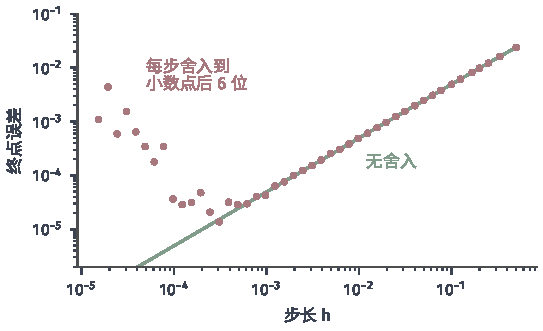
\includegraphics[width=92mm]{figures/06-differential-equations/01-ordinary-differential-equations/matplotlib/odenum-roundoff-v/figure.pdf}
 \caption{显式Euler方法的截断误差与舍入误差，问题为式~\eqref{eq:odenum-running}，$T=1$。绿线不作舍入，红点是每步把结果舍入到小数点后六位时的终点误差。$h$太大时截断误差主导，$h$太小时舍入误差累积主导。}
 \label{fig:odenum-roundoff-v}
\end{BookInlineFigure}

图中误差的最小值约为$10^{-5}$，出现在$h\approx3\times10^{-4}$附近，再缩小步长，误差反而变大。这比最坏情形的界算出的$h_{*}$更小，因为实际舍入有正有负、部分抵消，定理~\ref{thm:odenum-global-error}只给出上界。

\emph{真解在区间上不存在。}对$\dot{x}=x^2$，$x(0)=1$，解在$t=1$爆炸，定理的条件不成立。Euler方法却照常输出，取$h=0.5$走到$t=2$：
\[
 1,\quad 1.5,\quad 2.625,\quad 6.070,\quad 24.495.
\]
数值方法给出有限的数字，并不说明解在那里存在，第~\ref{chap:ode-existence-continuation}章的延拓判据不能省。

